\documentclass[english]{article}

%% Packages pull in extra commands:
%% http://en.wikibooks.org/wiki/LaTeX/Packages

\usepackage{hyperref}
\usepackage[letterpaper]{geometry}
\geometry{verbose,tmargin=1in,bmargin=1in,lmargin=1in,rmargin=1in}
\usepackage{amsmath}
\usepackage{amssymb}
\usepackage{graphicx}
\usepackage{float}
\usepackage{array}
\usepackage{tikz}
\usepackage{enumitem}
\usepackage{bbm}
\usepackage{xspace}
\DeclareMathOperator*{\argmax}{argmax}
\usepackage{spverbatim}

% New commands serve as shorthand for frequently used command combinations.
\newcommand{\ind}[1]{\mathbf{1}\left(#1\right)}
\newcommand{\bx}{\mathbf{x}}
\newcommand{\E}{\mathbf{E}}
\newcommand{\MATLAB}{\textsc{Matlab}\xspace}
\newcommand\scalemath[2]{\scalebox{#1}{\mbox{\ensuremath{\displaystyle #2}}}}

\title{CIS581: Computer Vision and Computational Photography\\Final Project\\Final Project Report}
\author{%
 \begin{tabular}{rl}
 Tianlin Du&(dtl1995) \tabularnewline
  Wentao He&(wentaoh) \tabularnewline
  Yezheng Li&(yezheng)
\end{tabular}
}

\begin{document}
\maketitle

\section{Introduction}
In this (short) project, we will implement vanilla recurrent neural networks (RNNs) and Long-Short Term Memory (LSTM) RNNs and apply them to image captioning on COCO.\\\\
Note: this project is adapted from the Standford CS231n course.

\section{Goal}
We will take a look at an interesting multi-modal topic where we will combine both image and text processing to build a useful Deep Learning application, aka Image Captioning. Image Captioning refers to the process of generating textual description from an image based on the objects and actions in the image.\\\\
Here are some examples of image captioning:\\\\
        \begin{figure}[H]
          \centering
          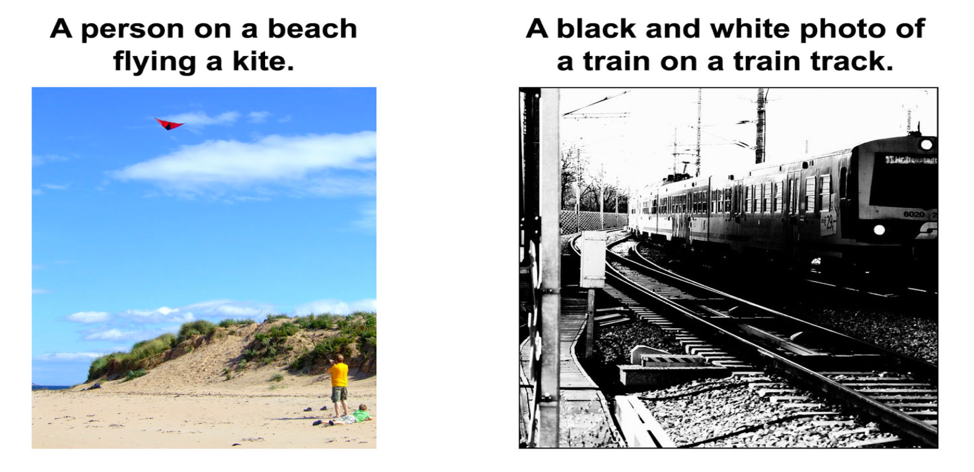
\includegraphics[width=0.6\textwidth]{Picture1.png}
          \caption{Image Caption Result 1}
        \end{figure}

\section{Implementation}
\begin{enumerate}
\item From the \texttt{RNN\_Captioning.ipynb} in Jupyter notebook, we implement the forward and backward pass for a vanilla RNN, first, 1) for a single timestep and then, 2) for entire sequences of data. Code to check gradients has already been provided. \\\\We overfit a captioning model on a tiny dataset and implement sampling from the softmax distribution and visualize predictions on the training and validation sets. The formula we used are shown below:
\begin{figure}[H]
          \centering
          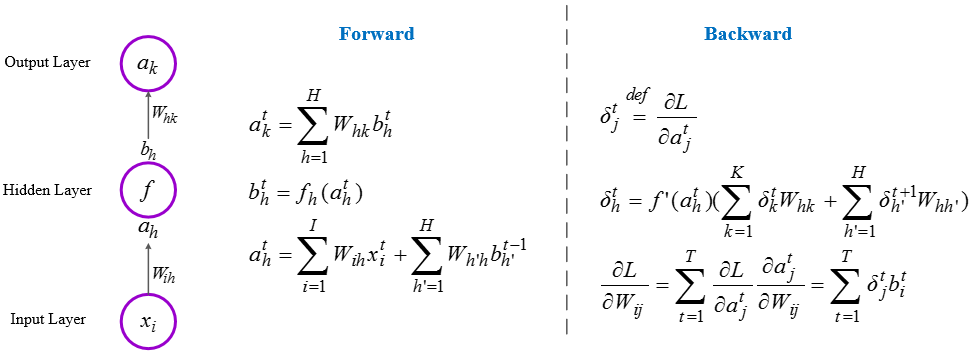
\includegraphics[width=0.6\textwidth]{Picture7.png}
          \caption{Forward and Backward Pass for a Vanilla RNN.}
\end{figure}
\item For a Recurrent Neural Network (RNN), a figure explaining its basic principle is shown below:
\begin{figure}[H]
          \centering
          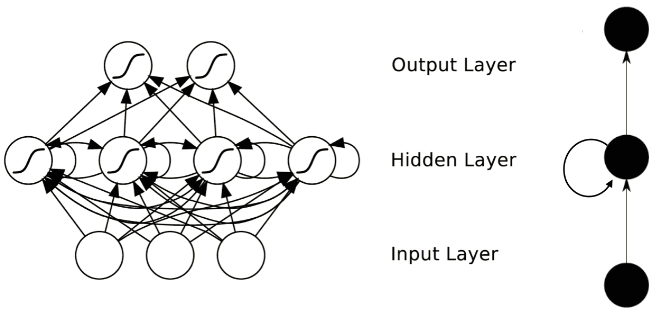
\includegraphics[width=0.6\textwidth]{Picture6.png}
          \caption{RNNs}
\end{figure}
\begin{figure}[H]
          \centering
          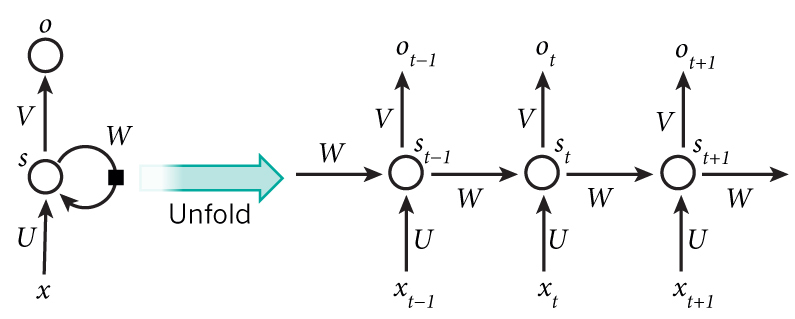
\includegraphics[width=0.6\textwidth]{Picture5.png}
          \caption{A RNN and the unfolding in time of the computation involved in its forward computation.}
\end{figure}
\item From the \texttt{LSTM\_Captioning.ipynb} Jupyter notebook, we implement Long-Short Term Memory (LSTM) RNNs, and apply them to image captioning on MS-COCO.
\begin{figure}[H]
          \centering
          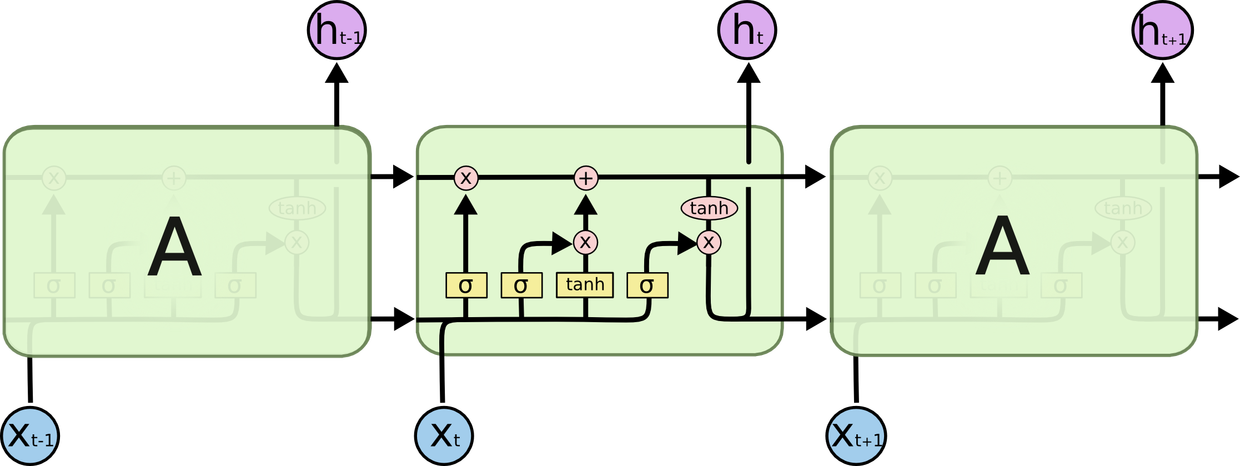
\includegraphics[width=0.6\textwidth]{Picture4.png}
          \caption{LSTM}
\end{figure}
\begin{figure}[H]
          \centering
          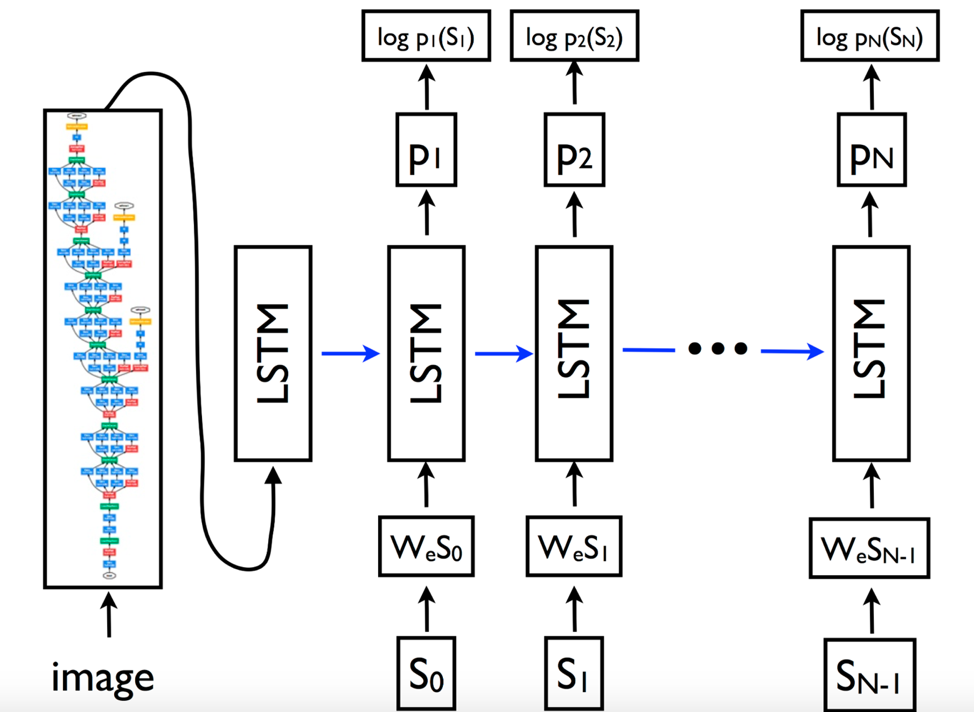
\includegraphics[width=0.6\textwidth]{Picture3.png}
          \caption{Long Short-Term Memory (LSTM) Network Decoder}
\end{figure}
\item Using the pieces we implement in parts 1 and 2, we train a captioning model that gives decent qualitative results (better than the random garbage you saw with the overfit models) when sampling on the validation set.
\end{enumerate}

\section{Results}

\section{References}
\begin{enumerate}
    \item Automatic Image Captioning using Deep Learning (CNN and LSTM) in PyTorch. \url{https://www.analyticsvidhya.com/blog/2018/04/solving-an-image-captioning-task-using-deep-learning/}.
    \item \url{https://github.com/tensorflow/models/tree/master/research/im2txt}.
    \item CS231n Convolutional Neural Networks for Visual Recognition. \url{http://cs231n.github.io/assignments2017/assignment3/}.
    \item Attention-based captioning models. \textit{[1, 7] Show, Attend and Tell: Neural Image Caption Generation with Visual Attention. Xu et al., 2015}. \url{https://arxiv.org/abs/1502.03044}.
\item \textit{Knowing When to Look: Adaptive Attention via A Visual Sentinel for Image Captioning. Lu et al., CVPR 2017}. \url{https://arxiv.org/abs/1612.01887}.
\item Discriminative captioning. \textit{Context-aware Captions from Context-agnostic Supervision. Vedantam et al., CVPR 2017}. \url{https://arxiv.org/abs/1701.02870}.
\item Novel object captioning. \textit{Deep Compositional Captioning: Describing Novel Object Categories without Paired Training Data. Hendricks et al., CVPR 2016}. \url{https://arxiv.org/abs/1701.02870}.
\item \textit{Captioning Images with Diverse Objects. Venugopalan et al., CVPR 2017}. \url{https://arxiv.org/abs/1701.02870}.
    \end{enumerate}

\end{document}
